\documentclass[twoside,11pt]{article}

\usepackage{jmlr2e}
\usepackage{natbib}
%\usepackage{parskip}
%\usepackage{float}

% Definitions of handy macros can go here
\newcommand{\dataset}{{\cal D}}
\newcommand{\fracpartial}[2]{\frac{\partial #1}{\partial  #2}}
% Heading arguments are {volume}{year}{pages}{submitted}{published}{author-full-names}

% Short headings should be running head and authors last names
\ShortHeadings{95-845: MLHC Article}{XIN GAO}
\firstpageno{1}

\begin{document}

\title{Heinz 95-845: Image Classification for Colorectal Cancer Diagnosis with CNN Model \\Machine Learning and Health Care}

\author{\name Xin Gao \email ANDREWID/xing1@andrew.cmu.edu \\
       \addr Heinz College\\
       Carnegie Mellon University\\
       Pittsburgh, PA, United States} 

\maketitle

\begin{abstract}

The aim of this project is to implement a Convolutional Neural Network (CNN) to extract distinctive features from the images of H&E stained colon tissue and predict the benign or malignant status for the sample. In this article, We will elaborate the ConvNet architecture which enabled an efficient training with an average accuracy over 80\% on test samples. In our model, we also chose a very popular optimizer Adam algorithm to better control the learning rate and minimize memory usage. 
 
\end{abstract}

\section{Introduction}
Image Classification is to assign an input image to a predefined fixed set of categories based on the identified representations. k-nearest neighbor (k-NN) and Support-Vector-Machine (SVM) are the most commonly adopted algorithms for classification. One of the most evident difference between these two approaches is that the former is a non-parametric classifier while the latter as learning-based classifier \citep{1}. Some research \citep{2}revealed that SVM outperformed k-NN on image datasets that have multiple attributes. One critical defect of k-NN is that it has a significantly high memory requirement to store all training images and high computation costs to compare test with all training images. SVM was considered to perform well on high-dimensional image datasets.

However, success in ImageNet competition in 2012 brought CNN in the spotlight and its substantially reduced top 5 error rate (15.4\% vs. the second best entry at 26.2\%) \citep{3}shocked the computer vision community. They began to realize the true value of CNN. Since then, CNN became increasingly popular and now as a state-of-art method to recognize objects, it has been widely applied in a variety of fields ranging from natural language processing to medical image analysis. As compared with other machine learning approaches, CNN is strong in extracting invariant image features through multiple stages, which enables CNN to learn representations of images more effectively.  

In this work, we will implement a CNN model on HE-stained colorectal images and make a prediction on whether the glands in a given image indicate a benign or malignant colon tumor. In the model, we created the basic building blocks for a simple ConvNet and explored Adam algorithm instead of the more commonly used stochastic gradient descent (SGD) to train the model. 

In Section 2, we provide background on colorectal cancer diagnosis based on histological image analysis and fundamental concepts to understand CNN architecture, such as convolutional layer, pooling layer, etc. In Section 3, we will deep dive into the model we built and go through each layer to understand how it works for classification. In the next Section, we will cover the data description, pre-processing process, method comparison and evaluation criteria. In Section 5, we will visualize some quantitative metrics to show how well our method works. In the last section, we will comprehensively evaluate our project in the following aspects including the contribution to existing research work, the limitations of our project and implications for clinical decision-making on colon cancer.

\section{Background} \label{background}
Colorectal cancer is the third most common cancan diagnosed in both men and women in the Unites States\citep{4}. H&E stained histological images are considered as one of the best way to detect the morphological features of glands. Over ninety percent of colorectal carcinomas could be categorized as adenocarcinomas, which are characterized by glandular morphology\citep{5}. Glandular malformation, in particular, the degree of differentiation from the normal glands determines the colon cancer grading. Detection and visual interpretation of morphological features largely affect pathologists' decision-making on whether the colorectal tumor is benign and malignant. Currently, pathologists are still playing a key role in manually reading and evaluating the images of HE-stained slides. One aim of our project is to automate this process and build a ConvNet to accurately discriminate benign cases from malignant cases. 

% insert a figure 1
\begin{figure}[!h]
\centering
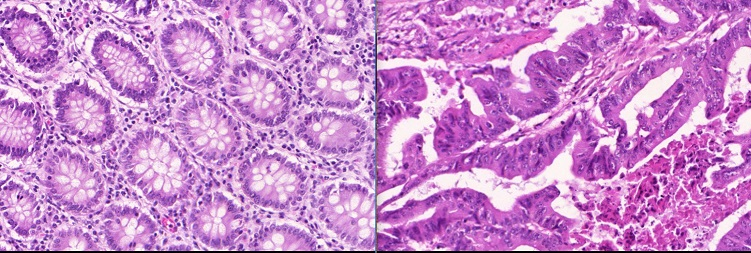
\includegraphics[width=.8\textwidth]{figure1.jpg}
\caption{Comparison of the Benign Case (left) and Malignant Case (right)}
\label{figure1}
\end{figure}

Different from a regular Neural Network, a neuron in ConvNet has three dimensions (width, height, depth). For RGB image the depth would be 3, but in our project, we use RGBA images and therefore the depth would be 4. There are three major types of layers in a ConvNet - convolutional layer, pooling layer and fully-connected layer. Through multiple layers, a ConvNet could eventually transform 3D-array pixel values of an image into a class score. 

In \textbf{convolutional layers}, a set of learnable filters (in tensorflow environment, it's also called kernel) slide across each small local regions of the input (or receptive field) and compute the dot product of the input and its weight to generate a 2D feature map (or activation map)\citep{6}. Every time the filter slides, the number of pixels it skips is called stride. For example, if the filter moves by 2 pixels, the stride equals to 2. The size of the receptive fields is regarded as the spatial extent of the filter. When the filter moves to the border, a zero will be added to the input array and this is called zero-padding. 

\textbf{Pooling layers} is added between convolutional layers to reduce volume size of the input. If we let the original size be W0*H0*D0, the number of filters be K, the spatial extent be F, the stride be S and the number of zero padding be P. 
Input volume would be:
\[
Input Volume = W0 *H0 *D0
\]
\[
Output Volume = W1 *H1 *D1
\]
\[
W1 = (W0 - F +2P)/S +1;
\]
\[
H1 = (H0 - F +2P)/S +1
\]
\[
D1 = K
\]
In addition, we applied a max filter to each non-overlapped receptive field to lower the dimensionalities, which is called max pooling

\textbf{Fully-connected layers} is connected to activations of each layer and used to compute the class score. Each image get a score for each class. We also added nonlinear activation function after fully-connected layer and in our model, we use ReLU to speed up the training
\[
relu(x) = max(0,x)
\]

Another concept to introduce is called \textbf{loss}. Take our project for example, if an image of a benign case gets a very high score for the label "malignant", it means it has a high (poor) loss. One of our aims is to minimize the loss and increase the accuracy. 
\[
loss = -log(P_j)
\]
The last component is the classifier. In our project, we used softmax function as the classifier, which generates the normalized probabilities. The function is written as: 
\[
	f_i(z) = {e^z}^j/\sum_{k}{e^z}^k
\]


\section{CNN Model} \label{model} 

% insert a figure 2
\begin{figure}[H]
\centering
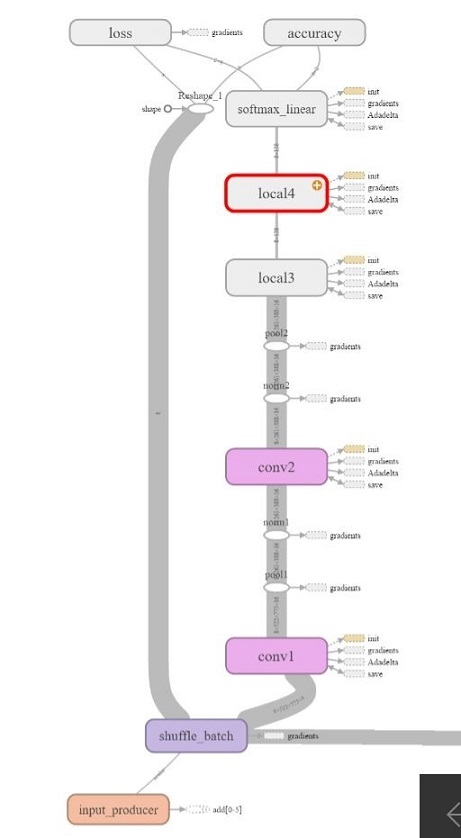
\includegraphics[width=.8\textwidth]{figure2.JPG}
\caption{CNN Model used in this Project)}
\label{figure2}
\end{figure}

We built seven layers to create the simple ConvNet architecture (Please refer to figure 3 on the next page). The architecture is as follows:
\[
INPUT -> CONV (+RELU) ->POOL -> CONV2(+RELU) ->POOL2 -> FC(+RELU) *2  -> SOFTMAX ->OUTPUT
\]

\textbf{Convolution Layer} We set the number of filters at 16, spatial extent at 3 and stride at 1. A total of two convoluational layers are implemented in this model for learning features.

\textbf{Pooling Layer} We added a local response normalization layer after pooling layer. The normalization layer works as a "lateral inhibition" to normalize the local neighbourhood of the excited neuron and better detect the features. In addition, 3*3 receptive fields are used for both pooling layers and 2*2 stride for the first one and 1*1 for the second one.

\textbf{Full-connected layer} Two full-connected layers are placed before the softmax function

\textbf{ReLU layers} ReLU is used as activation function throughout all layers

\textbf{Training} We chose Adam algorithms as the optimizer which requires less tuning parameter to perform well.Currently, it is recommended as the default optimizer to improve working efficiency and lower training costs \citep{7}. The optimizer is used to minimize the loss function. In terms of setting learning rate, we set it at 0.0001. As a tricky hyperparameter, we cannot set it too high or too low. 

\textbf{Softmax} We chose softmax instead of SVM as the classifier and assigned value 0 for benign case and value 1 for malignant case.


\begin{table}[htbp]
  \centering 
  \begin{tabular}{lclc} 
   Layer Tyep & Configuration \\ 
    \hline \\[-11pt]
    Input & Size:775*522*4\\
    Convolution & K =16, F =3, S=1, D= 4\\
    Pooling & Max, F=3, S=2\\
    Convolution & K = 16, F=3, S=1, D=4 \\
    Pooling & Max, F=3, S=1\\
    CF & \\
    SoftMax & \\
    Loss & Negative Log-likelihood \\\hline
  \end{tabular}
  \label{tab:example} 
    \caption{Architecture of Our Model} 
\end{table}

\section{Experimental Setup} \label{experiment}
\subsection{Cohort Selection} 
The dataset consists of 165 images of HE-stained colorectal adenocarcinoma in the format of BPM. All the datasets were acquired from the University of Warwickshire, UK. The table below shows the composition of the datasets in details.

\begin{table}[htbp]
  \centering 
  \begin{tabular}{lclc} 
    Histologic Grade & Training Set (Width*Height) & Test Set A (W*H)& Test Set B(W*H) \\ 
    \hline \\[-11pt]
    Benign & 1(574*433) & 2(574*433) & 4 (775*522) \\ 
           & 1(589*453) & 4(589*453) & \\
           &35(775*522) &28(775*522) & \\
    Total(Benign) & = 37       & =34        & = 4 \\ \hline
    Malignant & 1(567*430) & 1 (578*433) & 16(755*522) \\
              & 3(589*453) & 2 (581*422) & \\
              & 44(755*522) & 24 (755*522) & \\
    Total(Malignant) & = 48 & =27 & =16\\ \hline 
  \end{tabular}
  \label{tab:example} 
    \caption{Details of the Dataset} 
\end{table}

\subsection{Data Preprocessing} 
As shown in the table above, it's easily observed that images are in different widths and heights. Therefore, we resized them to ensure they have consistent width and height. Given that the size of the majority images is 755*522 in pixels, we decided to set the target width and height at (722,522). For those images with smaller size, we padded them evenly with zeros and then do normalization for each pixel. Different from the normal RGB images, we have to reset the shape of the images to ensure it has four channels. 

Secondly, CNN performs better on a large-scale dataset and given that we only have 85 images in the training set, we did the data augmentation to improve its performance. In this model, we use random flip function to horizontally and vertically flip the images. 

In addition, because tensorflow3.5 is applied to build the CNN model, we need to use a pipeline to read image files and convert input data into a 4-d tensor which has a shape of [batch, height, width, channels].

\subsection{Feature Choices} 
The format of images is BMP which could not be decoded or processed by tensorflow and therefore we converted them into BNP format. Another important feature is that our images have four channels, indicating that if we want to leverage existing well-trained model like VGG16, we may have to convert them into RBG images. 

\subsection{Comparison Methods}
We use a classic LeNet-5 architecture to built a seven-layer ConvNet. In vision4GlaS' model\citep{8}, they also used a seven-layer architecture to do a classification but they had three convolutional layers and only one fully connected layer. The table below shows key performance metrics for their model

\begin{table}[htbp]
  \centering 
  \begin{tabular}{lclc} 
    Dataset & Precision & Recall \\ 
    \hline \\[-11pt]
    Training & 0.97 (0.09) & 0.67(0.21) \\ 
    Test A    & 0.83 (0.22) & 0.60(0.24) & \\
    Test B    &0.70(0.35) & 0.48(0.30) & \\ \hline
  \end{tabular}
  \label{tab:example} 
    \caption{Performance Metrics of vision4GlaS' Model} 
\end{table}


\subsection{Evaluation Criteria}
To fine-tune our hyperparameters, we conducted a 5-fold cross-validation (ratio = 0.2). We split the training dataset into 5 equal folds and use 1 fold for validation.

Accuracy: orange line represents the training set and green line represents the validation set

% insert a figure 3
\begin{figure}[htbp]
\centering
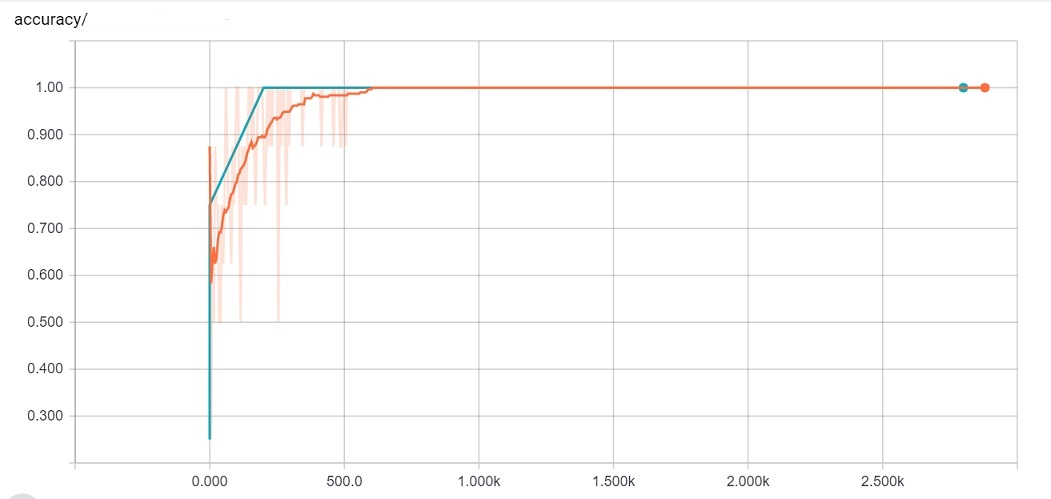
\includegraphics[width=.8\textwidth]{figure5.jpg}
\caption{Evaluation on Accuracy for Training and Validation Datasets)}
\label{figure1}
\end{figure}

Loss Reduction: orange line represents the training set and green line represents the validation set
(see figure 4 on the next page)

% insert a figure 4
\begin{figure}[htbp]
\centering
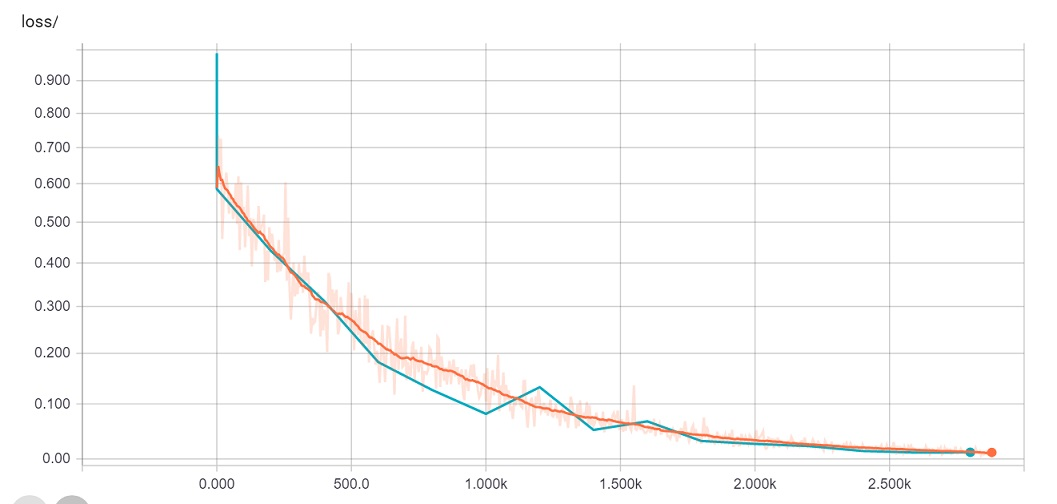
\includegraphics[width=.8\textwidth]{figure6.jpg}
\caption{Evaluation on Loss Reduction for Training and Validation Datasets)}
\label{figure1}
\end{figure}

\newpage
\section{Results} \label{results}
We predicted the accuracy on test samples and the table below shows the accuracy for test subset A and B. The average accuracy for test set A is 0.8179 and for test B is 0.8406.

\begin{table}[htbp]
  \centering 
  \begin{tabular}{lclc} 
    Test Subset & A& B \\ 
    \hline \\[-11pt]
    Mean & 0.8179&0.8406\\
    SE Mean & 0.0209 &0.8406\\
    StDev & 0.1436 & 0.1354\\
    Min & 0.5122 & 0.5619\\
    Median & 0.8930 &0.9078\\
    Max & 0.8930 &0.9078\\\hline
  \end{tabular}
  \label{tab:example} 
    \caption{Evaluation on Accuracy on Test Samples} 
\end{table}

% insert a figure 5
\begin{figure}[htbp]
\centering
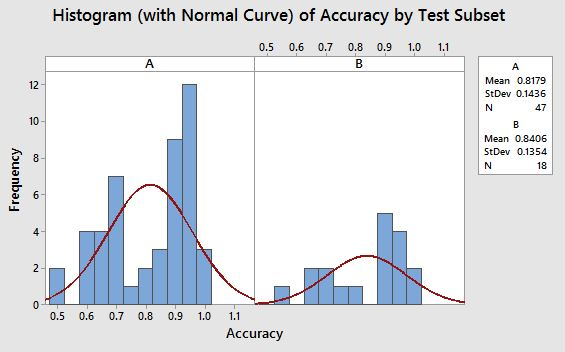
\includegraphics[width=.8\textwidth]{figure9.JPG}
\caption{Evaluation on Accuracy on Test Samples}
\label{figure1}
\end{figure}

\newpage
\section{Discussion and Related Work} 
In this project, we implemented a typical ConvNet model to classify the images of H&E-stained adenocarcinoma and achieved an accuracy over 80\%. However, there are many areas to be improved. 

Firstly, I may explore more advanced or novel CNN model. In H Chen, XJ Qi, et al \citep{9} (who is the winner of the competition)'s model, they used fully convolutional networks to conduct the image segmentation which achieved an F1 score of 0.9116 on test set A and 0.7158 on test set B. Their model contains two modules - down-sampling path and up-sampling path. The former includes convolutional layer and pooling layers and the latter includes convolutional layers and deconvolutional layers. 
Secondly, in terms of data pre-processing, I should do more testing to select the best target width and height. Some studies applied an equal target width and height at 480,480. 
Thirdly, due to the limitation of my computer's computational and storage capability, I could not add more layers to build a more complicated structure. Fourthly, the ultimate goal of this project is to use advanced machine learning algorithms to perform gland segmentation and depict gland contours. Tensorflow has released a new package TF-slim which is specialized in conducting image segmentation. Other computer vision packages like openCV could also be used to match the representative gland structure on the image and do the segmentation. Lastly, I need to use more metrics to evaluate the performance of the model like precision, recall, etc.

This project enables the automatic detection of a malignant colorectal tumor with a relatively good accuracy. This would help reduce the workload of clinical pathologists and serve as an auxiliary tool to improve diagnosis accuracy. 

\section{Conclusion} 
This project implemented a classic CNN model to distinguish benign colorectal adenocarcinoma from the malignant. We used seven layers to build the architecture and achieved a good accuracy on test samples. in future work, we will further optimize the method and investigate more novel algorithms to perform gland segmentation. 

\bibliography{sample}
\bibliographystyle{plainnat}

\newpage
\appendix
\section*{Appendix A.}
% insert a figure 6
\begin{figure}[htbp]
\centering
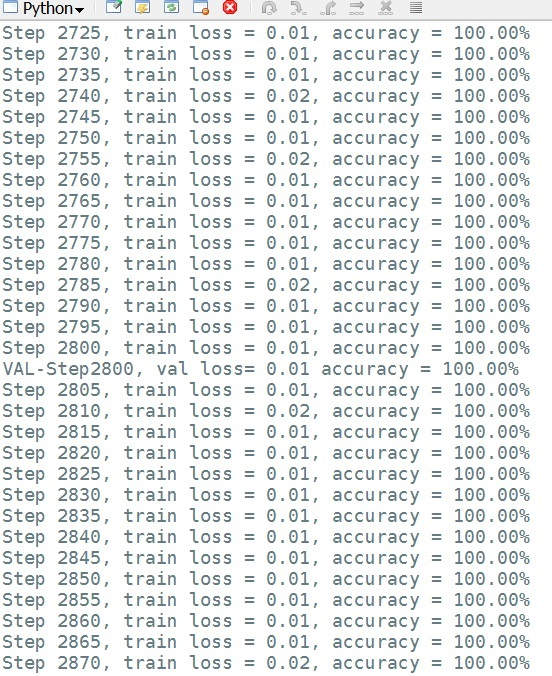
\includegraphics[width=.8\textwidth]{figure7.jpg}
\caption{Screenshot of Accuracy Evaluation}
\label{figure1}
\end{figure}


% insert a figure 7
\begin{figure}[htbp]
\centering
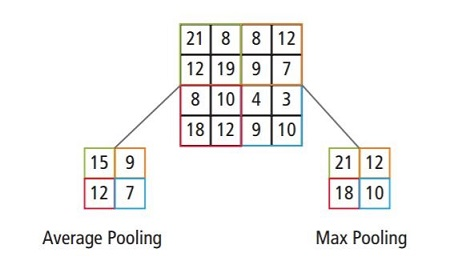
\includegraphics[width=.8\textwidth]{figure4.JPG}
\caption{Max Pooling vs. Average Pooling }
\label{figure1}
\end{figure}

% insert a figure 8
\begin{figure}[htbp]
\centering
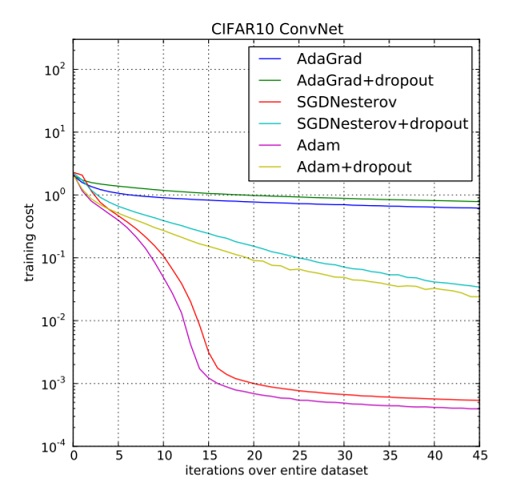
\includegraphics[width=.8\textwidth]{figure3.jpg}
\caption{Comparison of Different Optimizer in Reducing Training Costs}
\label{figure1}
\end{figure}

\end{document}
